\documentclass{beamer}
\usetheme{Boadilla}
\usepackage[cache=false]{minted}
\usepackage{multicol}
\usepackage{latexsym}
\usepackage{amsmath}
\usepackage{amssymb}
\usepackage{graphicx}

\graphicspath{{./images/}}
\newcommand\id{\mathsf{id}}
\newcommand\return{\mathsf{return}}
\newcommand\bind{\mathsf{>\!\!>\!\!=}}
\newcommand\app{\mathsf{<\!\!*\!\!>}}
\newcommand\unit{()}
\newcommand\pure{\mathsf{pure}}
\newcommand\fmap{\mathsf{fmap}}
\newcommand\join{\mathsf{join}}
\newcommand\oo{\ensuremath{\,\circ\,}}
\newcommand\om{\ensuremath{\,\odot\,}}
\newcommand{\M}[1]{\ensuremath{\mathsf{M}\,#1}}
\newcommand{\F}[1]{\ensuremath{\mathsf{F}\,#1}}
\newcommand{\A}[1]{\ensuremath{\mathsf{A}\,#1}}


\begin{document}
\titlegraphic{\vspace{-3em}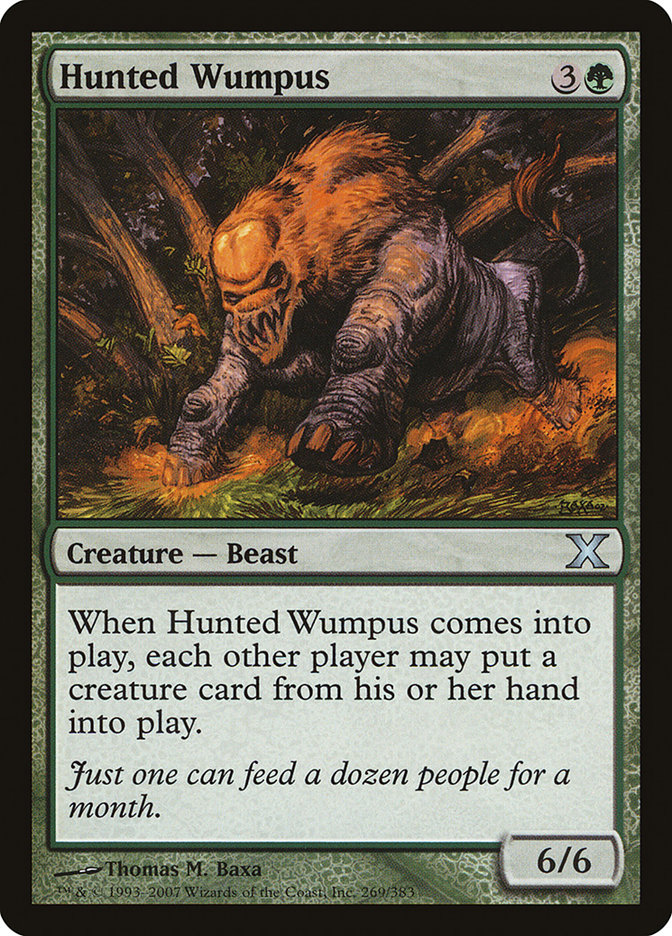
\includegraphics[width=.3\textwidth]{hunted-wumpus.jpg}}
\title{Hunt the Trevor}
\author{Elliot Greenwood}
\date{}
  \begin{frame}[fragile]
    \titlepage%
  \end{frame}
  \begin{frame}{Agenda}
    \begin{columns}[t]
      \begin{column}{.4\textwidth}
        \tableofcontents[sections={1-2}]
      \end{column}
      \begin{column}{.4\textwidth}
        \tableofcontents[sections={3-5}]
      \end{column}
    \end{columns}
  \end{frame}
  \section{What is a Monad?}
  \subsection{Intuition}
  \begin{frame}[fragile]{What is a Monad? (Recap)}{Intuition}
    Let's make a program
    
    \begin{minted}{haskell}
      main = do putStrLn "What is 2 + 2?"
                x <- readLn
                if x == 4
                    then putStrLn "You're right!"
                    else putStrLn "You're wrong!"
    \end{minted}
  \end{frame}
  \subsection{Theory}
  \begin{frame}{What is a Monad? (Recap)}{Theory}
    \begin{block}{Functor Definition}
      \begin{align*}
        \fmap &:: \mathbf{Functor}\ \mathsf{F}\ \Rightarrow\ (a\ \rightarrow\ b)\ \rightarrow\ \F{a}\ \rightarrow\ \F{b}\\
      \end{align*}
    \end{block}
    \begin{block}{Applicative Definition}
      \begin{align*}
        \pure &:: \mathbf{Applicative}\ \mathsf{A}\ \Rightarrow\ a\ \rightarrow\ \A{a}\\
        (\app) &:: \mathbf{Applicative}\ \mathsf{A}\ \Rightarrow\ \A{(a\ \rightarrow\ b)}\ \rightarrow\ \A{a}\ \rightarrow\ \A{b}\\
      \end{align*}
    \end{block}
  \end{frame}
  \begin{frame}{What is a Monad? (Recap)}{Theory}
    \begin{block}{Monad Definition}
      \begin{align*}
        \return &:: \mathbf{Monad}\ \mathsf{M}\ \Rightarrow\ a\ \rightarrow\ \M{a}\\
        (\bind) &:: \mathbf{Monad}\ \mathsf{M}\ \Rightarrow\ \M{a}\ \rightarrow\ (a\ \rightarrow\ \M{b})\ \rightarrow\ \M{b}\\
      \end{align*}
    \end{block}
    \begin{itemize}
      \item $\return$ constructs the monad\\
      \item $\bind$ allows composition of the monad\\
      \item Note: You might see other people say you need $\join$ to define the monad,
        providing either $\bind$ or $\join$ is ``rigorously'' equivalent.
    \end{itemize}
  \end{frame}

  \section{Reader}
\subsection{Motivation}
\begin{frame}[fragile]{Reader Monad}{Motivation}
  \begin{columns}[t]
    \begin{column}{.4\textwidth}
      {\tiny\inputminted[escapeinside=\\`\\`]{haskell}{reader-motivation.hs}}
    \end{column}
    \begin{column}{.4\textwidth}
      \begin{itemize}
        \item Notice how we must pass this \texttt{\mylib{wc}} around
        \item We must pass it through functions that may never use it
      \end{itemize}
    \end{column}
  \end{columns}
\end{frame}
\subsection{Definition}
\begin{frame}[fragile]{Reader Monad}{Type}
  \inputminted[escapeinside=||,fontsize=\tiny]{haskell}{reader-types.hs}
  {
    \vspace*{-4cm}
    \hspace{7cm}
    \begin{minipage}{.35\textwidth}
      \begin{tcolorbox}[colframe=gray,colback=white,boxrule=1pt,arc=3.4pt,boxsep=0mm]
        \begin{minted}{csharp}
          class Reader<TC, TA> {
            Reader(T runReader) {
              this.runReader = runReader;
            }
          }
        \end{minted}
      \end{tcolorbox}
    \end{minipage}%
  }
  \vspace*{2.5cm}
  \begin{block}{\textbf{Exercise: }Reader Type Definition}
    \begin{align*}
      \mathsf{newtype}\ \ReaderH{a} &=
        \mathsf{Reader} \left\{ \fn{runReader} ::\ \uncover<2->{\mylib{c}\ \rightarrow\ \mylibo{a}} \right\}\\
    \end{align*}
  \end{block}
\end{frame}
\begin{frame}[fragile]{Reader Monad}{Type}
  Recall: $\mathsf{newtype}\ \Reader{a} = \mathsf{Reader} \left\{ \fn{runReader} ::\ c\ \rightarrow\ a \right\}$
  \begin{block}{\textbf{Exercise: }Reader Type Definition}
    \begin{align*}
      \return &:: a\ \rightarrow\ \Reader{a}\\
      \return\ a\ &= \uncover<2->{\mathsf{Reader}\ (\lambda\,\underline{\phantom{c}}\ \rightarrow\ a)}\\[1.5em]
      (\bind) &:: \Reader{a}\ \rightarrow\ (a\ \rightarrow\ \Reader{b})\ \rightarrow\ \Reader{b}\\
      x\ \bind\ fn &=\uncover<3->{\mathsf{Reader}\ (\lambda\,c\ \rightarrow
      \fn{runReader}\ (fn\ (\fn{runReader}\ x\ c))\ c)}\\
    \end{align*}
  \end{block}
\end{frame}
\begin{frame}[fragile]{Reader Monad}{Functions}
    \begin{block}{\textbf{Homework: }Reader Functions}
      \begin{align*}
        \fn{ask} &:: \Reader{a}\ \rightarrow\ a\\
        \fn{asks} &:: \Reader{a}\ \rightarrow\ (a\ \rightarrow\ \Reader{b})\ \rightarrow\ \Reader{b}\\
        \fn{local} &:: (c\ \rightarrow\ c\,')\ \rightarrow\ \mathbf{Reader}\,c\,'\,a\ \rightarrow\ \Reader{a}\\
      \end{align*}
    \end{block}
\end{frame}
\subsection{Example}
\begin{frame}
  \centering
  \begin{tcolorbox}[enhanced, size=minimal,auto outer arc,
    width=2.8cm,octogon arc, colback=red,colframe=white,colupper=white, fontupper=\fontsize{7mm}{7mm}\selectfont\bfseries\sffamily, halign=center,valign=center,
    square,arc is angular, borderline={1mm}{-3mm}{red} ]
    CODE
  \end{tcolorbox}
\end{frame}
%
  \section{Writer}
\subsection{Motivation}
\begin{frame}[fragile]{Writer Monad}{Motivation}
  {\tiny\inputminted[escapeinside=||,breakafter=\$]{haskell}{writer-motivation.hs}}
  \begin{itemize}
    \item Notice how we must add onto this list of strings
    \item Functions don't care about the logs from what proceeded them, so why should we have to know about them
  \end{itemize}
\end{frame}
\subsection{Definition}
\begin{frame}[fragile]{Writer Monad}{Type}
    {\scriptsize\inputminted[escapeinside=||]{haskell}{writer-types.hs}}
    \begin{block}{\textbf{Exercise: }Writer Type Definition}
      \begin{align*}
        \mathsf{writer}\ \WriterH{a} &= \mathsf{Writer} \left\{ \fn{runWriter} ::\ \uncover<2->{(\mylib{$[\ell]$}, \mylibo{a})} \right\}\\
      \end{align*}
    \end{block}
\end{frame}
\begin{frame}[fragile]{Writer Monad}{Type}
  Recall: $\mathsf{writer}\ \Writer{a} = \mathsf{Writer} \left\{ \fn{runWriter} ::\ ([\ell], a) \right\}$
  \begin{block}{\textbf{Exercise: }Writer Type Definition}
    \begin{align*}
      \return &:: a\ \rightarrow\ \Writer{a}\\
      \return\ a\ &= \uncover<2->{\mathsf{Writer}\ ([\,], a)}\\[1.5em]
      (\bind) &::
      \begin{aligned}[t]
        \Writer{a}\ \rightarrow\ &{\text{\small\color{gray}\carriagereturn}}\\(a\ \rightarrow\ &\Writer{b})\ \rightarrow\ \Writer{b}
      \end{aligned}\\
      x\ \bind\ fn &=\uncover<3->{\mathsf{Writer}\ (
          \begin{aligned}[t]
            \mathbf{let}&\ 
            \begin{aligned}[t]
              (l, a) &= \fn{runWriter}\ x\\
              (l\,', b) &= \fn{runWriter}\ (fn\ a)
            \end{aligned}\\
            \mathbf{in}&\ (l\!\mappend\!l\,', b))
          \end{aligned}}\\
    \end{align*}
  \end{block}
\end{frame}
\begin{frame}[fragile]{Writer Monad}{Monoid}
  Let: $\mathsf{writer}\ \WriterM{a} = \mathsf{Writer} \left\{ \fn{runWriter} ::\ (\ell, a) \right\}$
  \begin{block}{\textbf{Exercise: }Writer Type Definition}
    \begin{align*}
      \return &:: a\ \rightarrow\ \WriterM{a}\\
      \return\ a\ &= \mathsf{Writer}\ (\fn{mempty}, a)\\[1.5em]
      (\bind) &::
      \begin{aligned}[t]
        \WriterM{a}\ \rightarrow\ &{\text{\small\color{gray}\carriagereturn}}\\(a\ \rightarrow\ &\WriterM{b})\ \rightarrow\ \WriterM{b}
      \end{aligned}\\
      x\ \bind\ fn &=\mathsf{Writer}\ (
          \begin{aligned}[t]
            \mathbf{let}&\ 
            \begin{aligned}[t]
              (l, a) &= \fn{runWriter}\ x\\
              (l\,', b) &= \fn{runWriter}\ (fn\ a)
            \end{aligned}\\
            \mathbf{in}&\ (\fn{mappend}\ l\ l\,', b))
          \end{aligned}\\
    \end{align*}
  \end{block}
\end{frame}
\begin{frame}[fragile]{Writer Monad}{Functions}
    \begin{block}{\textbf{Homework: }Writer Functions}
      \begin{align*}
        \fn{tell} &:: \ell\ \rightarrow\ \WriterM{\unit}\\
        \fn{censor} &:: (\ell\ \rightarrow\ \ell)\ \rightarrow\ \WriterM{a}\ \rightarrow\ \WriterM{a}\\
        \fn{listen} &:: \WriterM{a}\ \rightarrow\ \WriterM{(a, \ell)}\\
      \end{align*}
    \end{block}
\end{frame}
\subsection{Example}
\begin{frame}
  \centering
  \begin{tcolorbox}[enhanced, size=minimal,auto outer arc,
    width=2.8cm,octogon arc, colback=red,colframe=white,colupper=white, fontupper=\fontsize{7mm}{7mm}\selectfont\bfseries\sffamily, halign=center,valign=center,
    square,arc is angular, borderline={1mm}{-3mm}{red} ]
    CODE
  \end{tcolorbox}
\end{frame}

%
  \section{State}
\subsection{First Principals}
\begin{frame}

\end{frame}
\subsection{Definition}
\begin{frame}

\end{frame}
\subsection{Example}
\begin{frame}

\end{frame}
%
  \section{It's Trevor Hunting Time}
\begin{frame}[fragile]
  \fontsize{30pt}{1em}\selectfont
  \vspace*{-260pt}
  \hspace*{-225pt}
  \begin{tikzpicture}[scale=1.3, every shadow/.style={opacity=1,fill=blue!10!black}]
    \foreach \l in {300.8,280.8,...,60.8} {%
      \path[circular glow={shadow scale=1.03}, shading=radial, inner color=yellow!80!white, outer color=red!50!black] (0, 0) circle (\l pt);
    }

    \begin{scope}
      \path[circular glow={shadow scale=1.03}, shading=radial, inner color=blue!25!black, outer color=darkblueOuter,clip] (0, 0) circle (60pt)
      node[circle,inner sep=60pt,fill overzoom image=wumpus] at (0pt, -35pt) {};
    \end{scope}

    \node (b) at (-3, -0.8) {};
    \node (e) at (10, -1.2) {};
    \draw[decoration={text along path, text color=white, text={That's all Folks!}}, decorate] (b) to[bend left=15] (e);
  \end{tikzpicture}
\end{frame}
%
\end{document}
